\documentclass[a4paper]{report}
\usepackage[utf8]{inputenc}
\usepackage[T1]{fontenc}
\usepackage[english,main=french]{babel}
\usepackage[babel=true]{csquotes}
\usepackage{translator}
\usepackage{graphicx}
\usepackage{float}
\usepackage[export]{adjustbox}
\usepackage{amsmath}
\usepackage{amsfonts}
\usepackage{algorithm2e}
\usepackage{hyperref}
\usepackage{listings}
\usepackage{pgfgantt}
\usepackage[toc,page]{appendix}
\usepackage[backend=biber,style=alphabetic]{biblatex}
\usepackage{glossaries}
%\usepackage[top=2.5cm,bottom=2.5cm,left=3cm,right=2cm]{geometry}

\providetranslation[to=french]{April}{Avril}
\providetranslation[to=french]{May}{Mai}
\providetranslation[to=french]{June}{Juin}
\providetranslation[to=french]{July}{Juillet}
\providetranslation[to=french]{August}{Août}

\graphicspath{ {../images/} }
\bibliography{refs.bib}
\nocite{*}
\RestyleAlgo{ruled}
\renewcommand{\appendixpagename}{Annexes}
\renewcommand{\appendixtocname}{Annexes}
\hypersetup{
    colorlinks=true, %colorise les liens
    breaklinks=true, %permet le retour  la ligne dans les liens trop longs
    urlcolor=blue, %couleur des hyperliens
    linkcolor=black, %couleur des liens internes
    bookmarksopen=true, %si les signets Acrobat sont crs, les afficher compltement.
}
\lstset{
    basicstyle=\ttfamily,
    breaklines=true,
    showstringspaces=false,
    keywordstyle=\color{blue},
}


\title{Rapport de stage}
\author{Oscar Buon}


\begin{document}


\begin{titlepage}
    \centering
    \begin{minipage}{0.45\textwidth}
        
\includegraphics[width=\textwidth]{logo_ISIMA_INP.png}
    \end{minipage}\hfill
    \begin{minipage}{0.45\textwidth}
        
\includegraphics[width=\textwidth]{logo_CERN.png}
    \end{minipage}

    \vfill

    {\Large
        Rapport d'élève ingénieur \par
        Stage de 2ème année \par
        Filière 1 : Informatique des systèmes interactifs pour l’embarqué, la robotique et le virtuel \par
    }

    \vfill

    {\huge\bfseries Speeding up LHCb software through compilation optimization \par}

    \vfill

    {\Large Présenté par : Oscar Buon \par}

    \vfill

    \begin{minipage}{0.65\textwidth}
        \textsc{Responsable ISIMA : Mamadou Kanté}\\
        \textsc{Responsable Entreprise : Sébastien Ponce}\\
    \end{minipage}
    \hfill
    \begin{minipage}{0.25\textwidth}
        \textsc{4 septembre 2023} \\
        \textsc{Stage de 5 mois} \\
    \end{minipage}

    \vfill

    Campus des Cézeaux. 1 rue de la Chebarde. TSA60125. 63178 Aubière CEDEX
\end{titlepage}


\pagenumbering{Roman}
\chapter*{Remerciements}
J'aimerais commencer par remercier Sébastien Ponce, mon tuteur de stage sans qui mon travail au CERN n'aurait pas été possible et qui m'a aidé tout au long.

Merci également à M. Mamadou Kanté, tuteur ISIMA et responsable de la filière.

\bigskip
Je tiens aussi à remercier Alexandre Boyer qui m'a permis à l'occasion du forum ingénieur de trouver un stage au CERN.

\bigskip
Merci à Marco Clemencic qui m'a plusieurs fois aidé à résoudre certains problèmes.

\bigskip
Enfin je remercie Gloria Corti et Marco Cattaneo qui m'ont fait visité LHCb et DELPHI sous terre.

\tableofcontents

\listoffigures


\begin{abstract}
    Ce stage a pour objectif d'étudier l'infrastructure logicielle qui traite les données du détecteur LHCb du CERN et de mettre en place des solutions pour l'optimiser via une meilleure compilation.
    Les programmes sont principalement codés en C++ et compilés via CMake.

    Plusieurs méthodes ont été essayées.
    La première a été de fusionner les centaines de bibliothèques dynamiques en un seul exécutable.
    L'utilisation de profile-guided optimization et de link-time optimization a également été mise en place.
    Enfin les options \emph{fast-math} ont été testées.

    Une amélioration d'environ $11\%$ a été obtenue avec le link-time optimization, le profile-guided optimization et fast-math.

    \vfill

    Mots-clés : LHCb, Optimisation, Compilation avancée

\end{abstract}

\begin{otherlanguage}{english}
    \begin{abstract}

        \vfill

        Key words : LHCb, Optimization, Advanced compilation
    \end{abstract}
\end{otherlanguage}


\pagenumbering{arabic}
\chapter*{Introduction}
LHCb est l'une des quatre principales expériences du Large Hadron Collider (LHC) du CERN.
À l'intérieur se font plus de 30 millions de collisions par secondes, ce qui produit un flux de données d'environ $5 To/s$.
Ces données doivent rapidement être traitées pour reconstruire les trajectoires des particules et pour pouvoir être analysées tout autour du monde.

L'infrastructure logicielle de traitement est principalement écrite en C++ et en Python.
Du code est ajouté ou modifié tous les jours par plusieurs centaines de membres de la collaboration, qui représentent 83 instituts dans 19 pays en 2020.
Cela représente des millions de lignes de codes qu'il faut maintenir et améliorer.
Pour gérer cela, des outils modernes comme Git, gcc, clang ou CMake sont utilisés.

L'objectif du stage est d'abord de proposer et d'implémenter des solutions pour améliorer l'efficacité des programmes.
De plus, la mise en place de systèmes aidant au maintient de l'infrastructure peuvent être étudiés.

D'abord sera étudier la possibilité d'utiliser des \emph{bibliothèques statiques} à la place des \emph{dynamiques}.
Ensuite sera aborder la mise en place de \emph{profile-guided optimization} pour la compilation des programmes.
Aussi la mise en place d'outils permettant de mieux gérer les inclusions dans le code source sera envisagée.
Enfin sera étudier l'impact de l'utilisation du \emph{fast math} sur la rapidité et la stabilité des programmes.

La première partie de ce rapport est consacrée à l'étude et l'analyse des problèmes.
La seconde explique les méthodes et solutions techniques utilisées.
La dernière rend compte des résultats.


\chapter{Introduction}
\section{Présentation du CERN}
L'Organisation européenne pour la recherche nucléaire est le plus grand laboratoire d'étude de la physique des particules au monde.
Le centre, qui a été fondé en 1954, se situe sur la frontière franco-suisse à quelques kilomètres de Genève.

Une grande partie des recherches effectuées au CERN utilisent différents accélérateurs de particules.
Le principe est de faire atteindre à des particules des vitesses proches de celle de la lumière pour qu'elles acquièrent une grande énergie, puis de les faire entrer en collision.
La physique des particules prévoit alors l'apparition de nouvelles particules.
Ainsi en détectant les particles résultantes de ces collisions au seins de l'accélérateur et en comparant avec la théorie, on peut la valider ou l'invalider.

Il existe plusieurs accélérateurs et plusieurs expériences au CERN.
Le plus grand accélérateur est le Grand collisionneur de hadrons ou Large Hadron Collider (Figure \ref{LHC}) qui a été mis en fonction en 2008 et qui a une circonférence d'environ 27 kilomètres.
Il permet d'accélérer des protons à environ $7 Tev$.

\begin{figure}[!htb]
    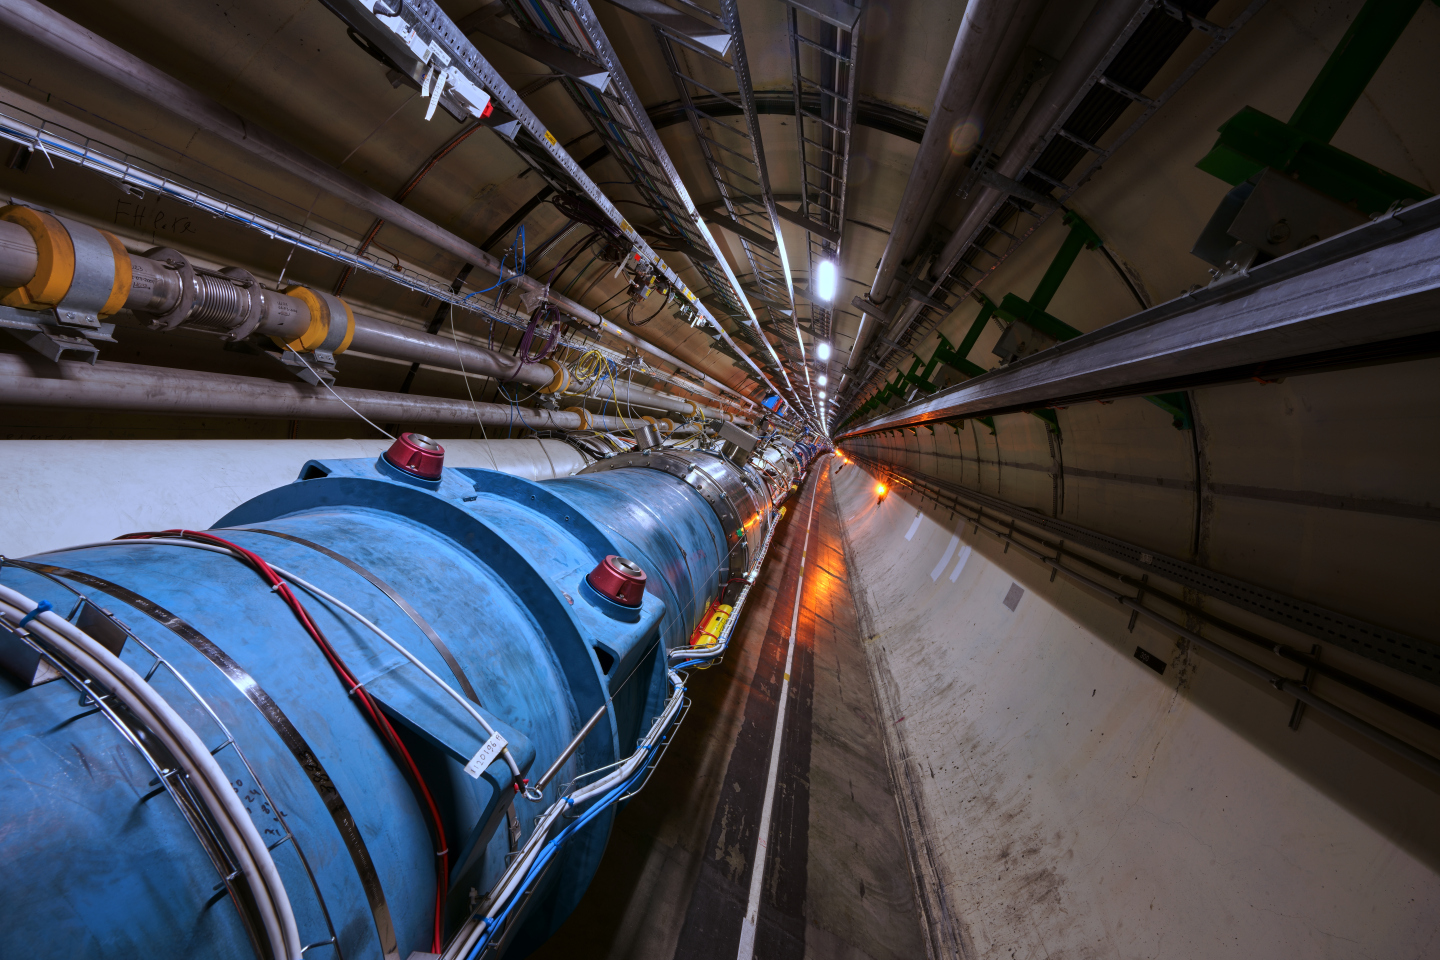
\includegraphics[width=\textwidth, center]{LHC.jpg}
    \caption{Tunnel du LHC}
    \label{LHC}
\end{figure}

Le CERN est connu pour être à l'origine de plusieurs découvertes importantes.
On peut notamment citer la découverte du boson de Higgs en 2012 qui a mené à 3 prix Nobels.
Le CERN est aussi à l'origine de la création du World Wide Web (Figure \ref{WEB}), qui permettait à l'origine le partage de papiers scientifiques.

\begin{figure}[!htb]
    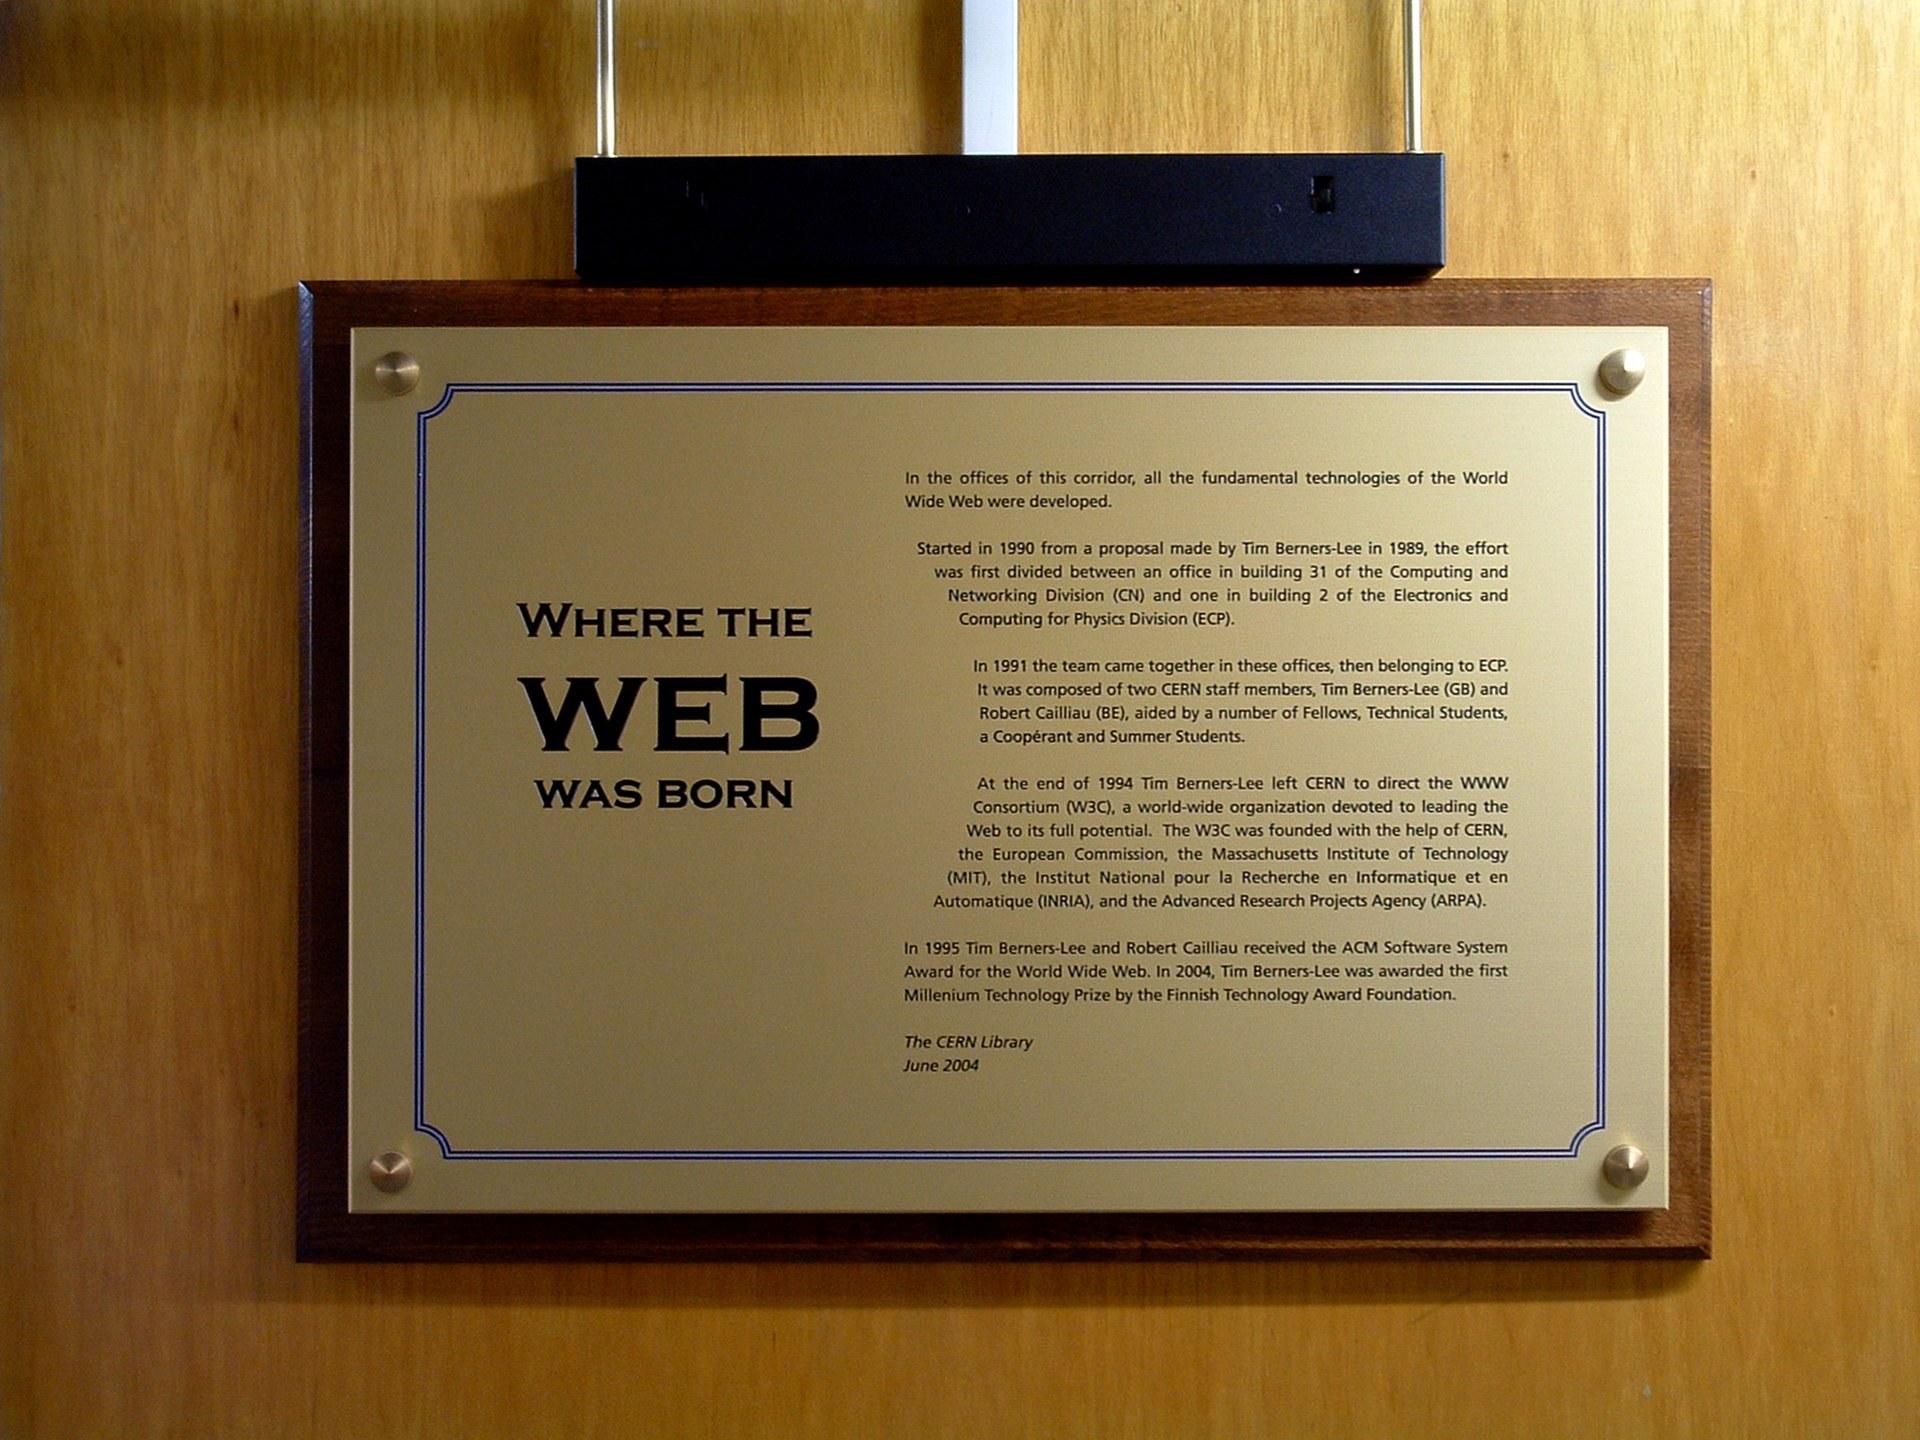
\includegraphics[width=\textwidth, center]{WEB.jpg}
    \caption{Plaque commémorative de l'invention du World Wide Web dans le bâtiment 1 du CERN}
    \label{WEB}
\end{figure}

Sur le LHC sont installés quatre principales expériences qui sont des collaborations internationales : ATLAS, CMS, ALICE et LHCb.
Ces expériences prennent la forme de détecteurs. C'est à l'intérieur d'eux que se font les collisions dont les résidus sont détectés par plusieurs types de capteurs.

La mise en oeuvre des expériences du CERN a depuis longtemps nécessité le développement de nouvelles technologies.
Ainsi l'informatique et internet sont présent depuis longtemps afin de gérer la masse de données produites dans les détecteurs \cite{Saikumar:2022mgb}.
Des programmes comportant plusieurs millions de lignes de codes sont exécutées aux centres de calcul sur les sites du CERN mais aussi partout autour du monde grâce au "Grid".
Le CERN a aussi contribué au développement d'internet en Europe.

\section{L'expérience LHCb}
Le Large Hadron Collider beauty (Figure \ref{LHCb}) est l'une des quatre principales expériences installées sur le LHC.
Elle vise l'étude du quark b afin de mesurer l'asymétrie entre matière et antimatière.
La collaboration regroupe plus de 1200 personnes représentant plusieurs dizaines d'instituts.
L'expérience se situe sur le point 8 du LHC.

\begin{figure}[H]
    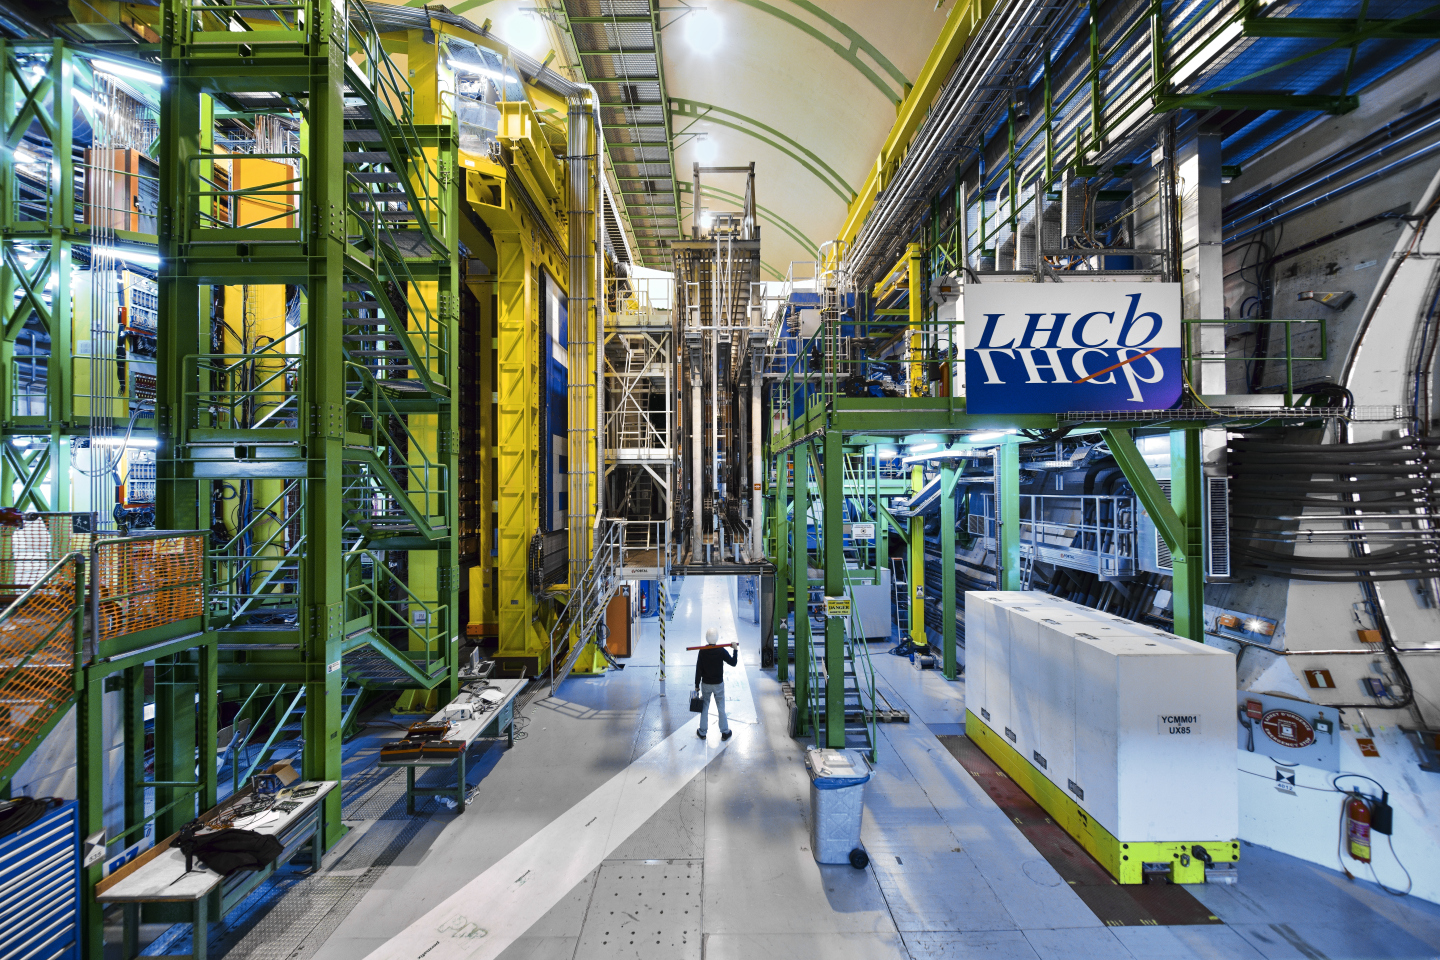
\includegraphics[width=\textwidth, center]{LHCb.jpg}
    \caption{LHCb}
    \label{LHCb}
\end{figure}

Le détecteur est composé de plusieurs instruments qui mesurent le passage des particules émises lors des collisions (Figure \ref{LHCb_3D}).
Grâce aux données recueillies, on peut reconstruire les trajectoires des particules ainsi que certaines de leur propriétés comme la masse ou la charge.

\begin{figure}[!htb]
    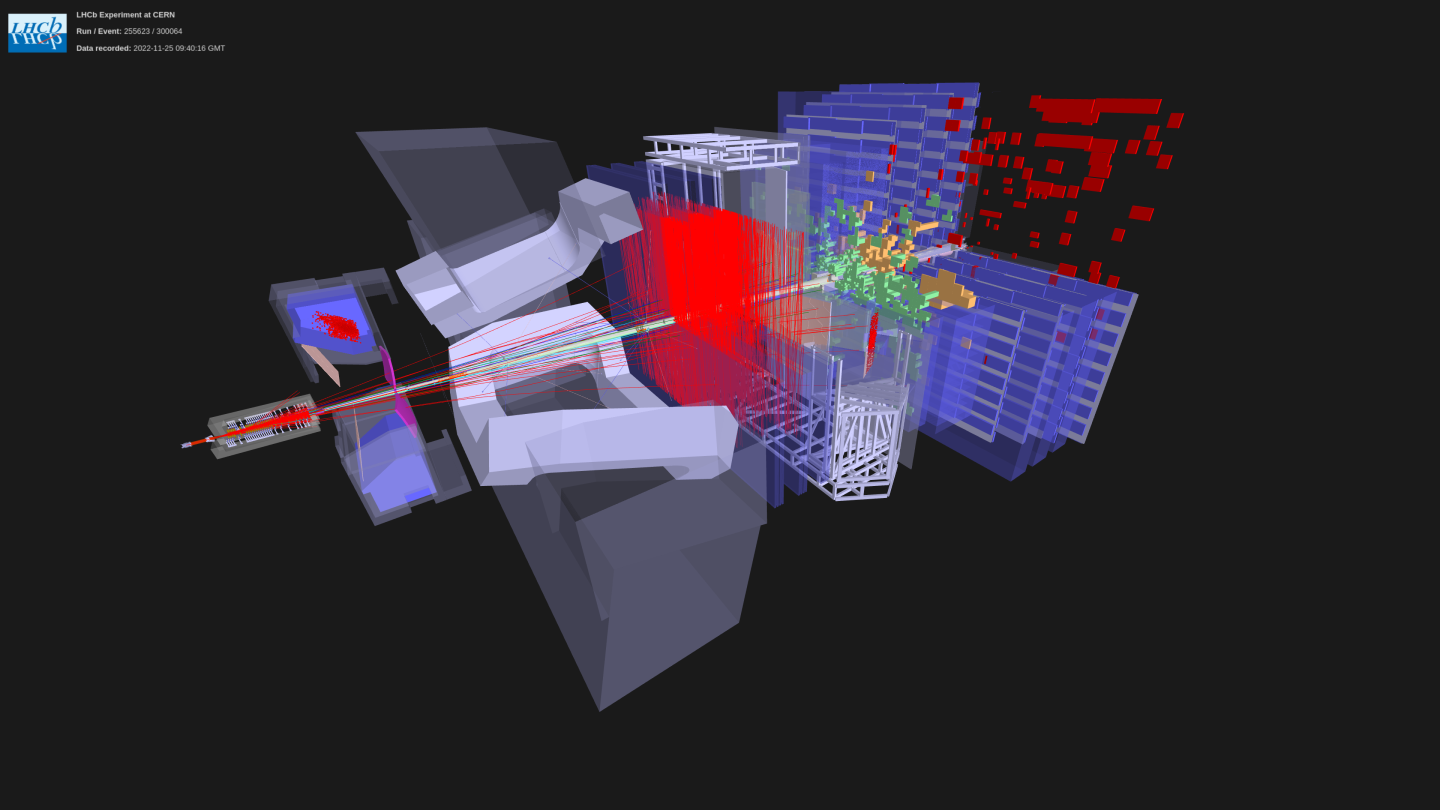
\includegraphics[width=\textwidth, center]{LHCb_3D.png}
    \caption{Modélisations de particules dans le détecteur}
    \label{LHCb_3D}
\end{figure}

\section{Computing Group}
Les différents instruments du capteur produisent un flux de données conséquent d'environ $5 To$ (Figure \ref{LHCb_stack}).
Une importante infrastructure informatique est donc nécessaire pour pouvoir les traiter.

\begin{figure}[!htb]
    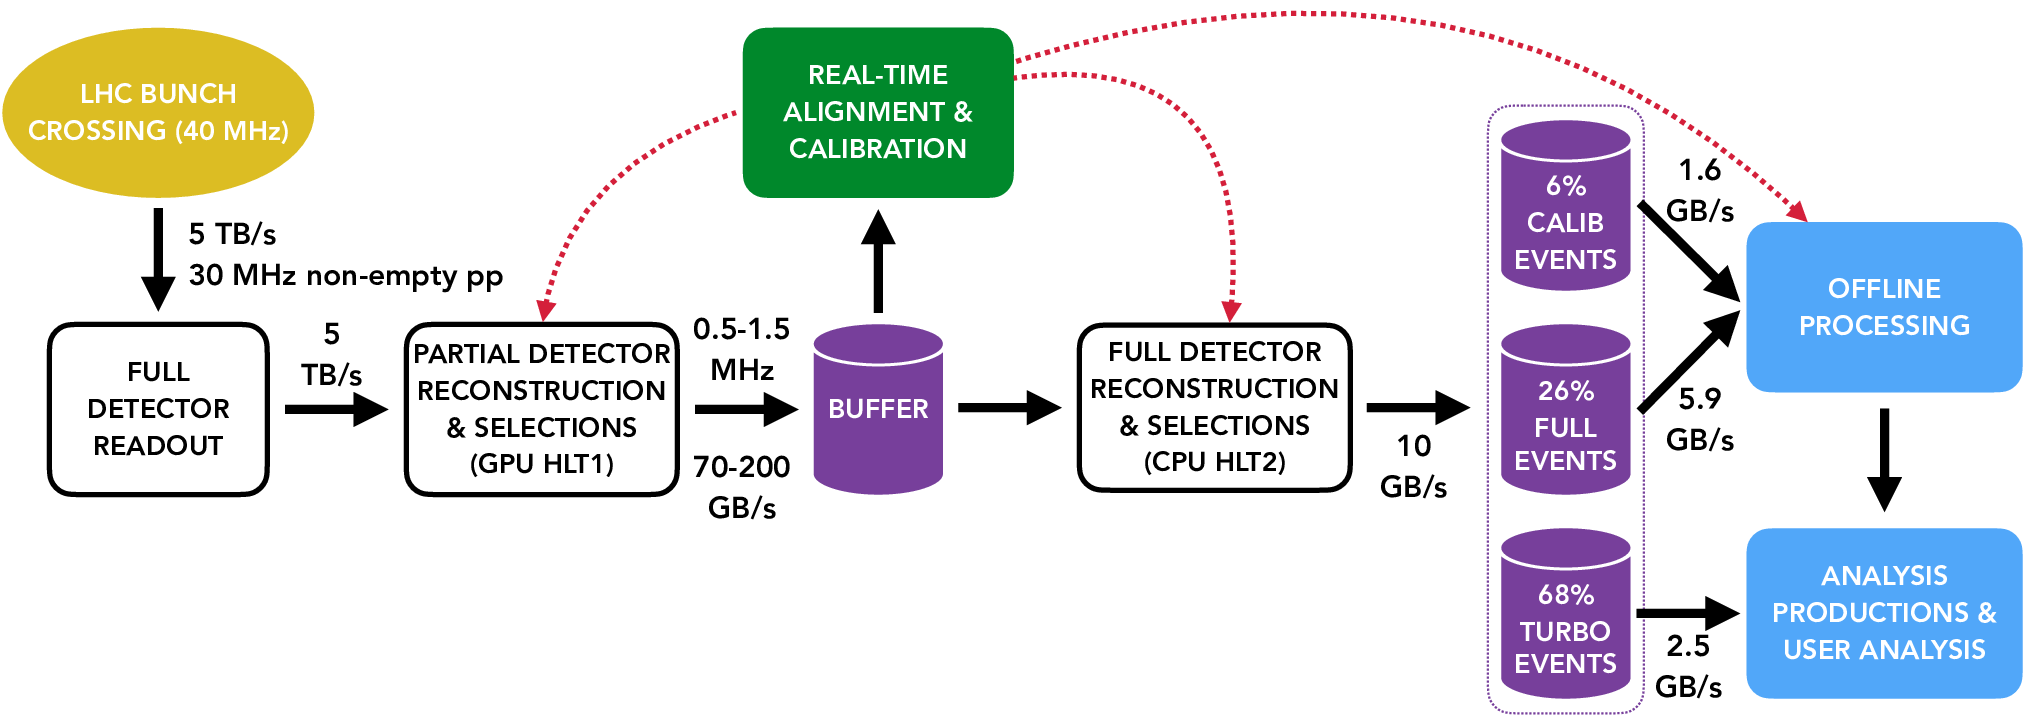
\includegraphics[width=\textwidth, center]{LHCb_stack.png}
    \caption{Infrastructure de gestion des données issues du détecteur}
    \label{LHCb_stack}
\end{figure}

LHCb utilise une pile de programmes (dont certains sont partagés avec d'autres expériences) qui traitent les données issues du détecteur.
Cette pile contient plusieurs millions de lignes de codes.
Ce code est principalement du C++ fait en grande partie par des physiciens non ingénieurs en informatique et dont certaines parties ont plusieurs décennies.

Son maintient et son amélioration est donc un enjeux majeur.
C'est le Computing Group du LHCb qui est chargée de cette tâche.

\section{Travail à faire et analyse}
Le code C++ de LHCb est compilé avec l'outil CMake qui permet de simplement définir les différentes cibles de compilation ainsi que leurs dépendances.
Il est composé de plusieurs programmes qui forment une pile.
On peut citer : Geant, Root, Gaudi qui sont partagés avec d'autres expériences et Detector, LHCb, Lbcom, Rec ou Moore qui sont spécifiquement pour LHCb.
Tout ceci tourne sur des serveurs Linux et est largement \emph{multithreadé}.

L'objectif de ce stage est d'implémenter des solutions pour améliorer la rapidité de l'exécution du code.
Les deux principales voies initialement envisagées sont l'utilisation de bibliothèques statiques à la place des dynamiques et la mise en place de profile-guided optimization.

\section{Étude et analyse des problèmes}

\subsection{Étapes de compilation}
Un programme écrit dans un langage de programmation comme le C ou le C++ ne peut pas être exécuté directement.
Pour ça, il doit d'abord être transformé en un fichier binaire exécutable par le système.
On appelle ce processus la compilation.
Le passage du code source au binaire final se fait en plusieurs étapes que voici :
\begin{enumerate}
    \item Le \emph{préprocesseur} exécute les macros et les autres directives pour modifier le code source.
    \item Le \emph{compilateur} fait l'analyse lexicale et syntaxique pour produire du code assembleur à partir du code source.
          Il peut également faire des optimisations.
          C'est l'étape la plus importante.
    \item L'\emph{assemblage} du code assembleur en fichiers objets.
          Cette étape est souvent fusionnée avec la précédente.
    \item Le \emph{linker} fusionne les fichiers objets en un binaire.
          Pour cela il fait la résolution des différents symboles utilisés.
\end{enumerate}

\subsection{Types de bibliothèques}
Il est possible de compiler du code C ou C++ non pas comme un exécutable mais comme une bibliothèque.
Cette bibliothèque peut ensuite être linkée avec un exécutable ou une autre bibliothèque afin de lui fournir des fonctions ou symboles.
Il existe plusieurs types de bibliothèques.

\subsubsection{STATIC}
Une bibliothèque statique est une archive de fichiers objets.
Lors du linkage avec un exécutable, ceux-ci sont simplement linkés avec les autres fichiers objets issus des fichiers sources du programme.

\subsubsection{SHARED}
Une bibliothèque partagée est un fichier compilé sous forme de bibliothèque externe.
On lui donne souvent l'extension \verb'.so' sous Linux ou \verb'.dll' sous Windows.
Ce fichier n'est pas linké après la compilation mais au chargement de l'exécutable par le \emph{linker dynamique} via une liste de dépendances que contient l'exécutable.

Comme leur nom l'indique, ces bibliothèque peuvent être partagées par plusieurs binaires.
Ainsi, si plusieurs exécutables utilisent la même bibliothèque partagée, il n'y a besoin de la compiler ou de la télécharger qu'une seule fois sur la machine.
De plus, il est possible de mettre à jour la bibliothèque sans avoir besoin de mettre à jour les exécutables.

\subsubsection{MODULE}
Un module est en fait une bibliothèque partagée, à la différence qu'on la charge manuellement pendant l'exécution, alors qu'une bibliothèque partagée est automatiquement linkée au démarrage.
Pour ce faire on utilise la fonction C \verb'dlopen' à laquelle on donne le chemin du module.

Ainsi les modules permettent de charger complètement dynamiquement des parties de programme selon les besoins.
Ils sont donc très utilisés dans LHCb afin de ne charger que ce qui est nécessaire pour effectuer les calculs demandés.

On peut aussi compiler et charger du code à la volée.
Ce mécanisme est utilisé dans LHCb via ce qu'on appelle les foncteurs.

\subsubsection{Cas de LHCb}
La pile LHCb est découpée en centaines de petites parties.
Ce découpage existe d'abord pour des raisons historiques car cela permettait de plus facilement collaborer sur le même projet avant l'arrivée de Git.
Mais cela permet aussi de ne pas avoir à tout compiler et charger lorsqu'on a besoin de travailler sur seulement certaines parties.

De ce fait la pile une fois compilée se compose de centaines de bibliothèques et de modules dynamiques.
Cette architecture est certes plus simple à utiliser mais il pourrait être intéressant d'étudier si leur fusion en un seul grand exécutable permettrait une meilleur performance en production.

\subsection{Guided optimization}
Les compilateurs comme \emph{gcc} ou \emph{clang} possèdent des options qui permettent de compiler un programme mieux optimisé.
Parmi ces optimisations on peut citer :
\begin{itemize}
    \item l'\emph{inlining} qui est le fait de remplacer l'appel d'une fonction par le corps de la fonction elle-même ;
    \item la réorganisation des blocs, par exemple lorsqu'il y a un branchement ;
    \item la mise en registre de certaines variables.
\end{itemize}
Certaines de ces optimisations utilisent des heuristiques pour déterminer quelle possibilité est la plus probable.
Tout ceci permet de multiplier les performances d'un programme compilé en mode optimisé.

Cependant les heuristiques utilisés sont quelques fois faux, ce qui représente un manque d'optimisation à gagner.
Pour pouvoir faire mieux, il faudrait pouvoir savoir comment le programme se comporte en situation réelle afin de mieux choisir pour chaque cas quelle est la meilleure solution d'optimisation.

\subsubsection{Profile-guided optimization}
Le \emph{profile-guided optimization} est une technique qui consiste à :
\begin{enumerate}
    \item compiler une première fois le programme avec des options pour faire de \emph{l'instrumentation} ;
    \item faire tourner le programme de manière classique afin que l'instrumentation crée \emph{profiles} sur le comportement du programme ;
    \item recompiler le programme en utilisant les profiles précédemment créés pour mieux optimiser dans les détails.
\end{enumerate}
Cette technique permet souvent d'obtenir un gain de performances situé entre $5\%$ et $10\%$ et a déjà été mise en place avec succés pour l'expérience CMS \cite{VIPGOforCMSReco}.

\subsubsection{Feedback directed optimization}
Cette solution proposée par Google \cite{45290} repose sur le même principe que le PGO à la différence que la première compilation n'a pas besoin de se faire avec des options d'instrumentation.
À la place, on utilise des outils de \emph{profiling} lors de l'exécution du programme pour créer les profiles.
Cette technique peut être plus facile à mettre en oeuvre et offre des résultats sensiblement similaires.

\subsubsection{Link-time optimization}
Lorsqu'on compile un programme C ou C++, on compile indépendamment chaque fichier source (\emph{translation unit}) en fichier objet.
Ces fichiers sont ensuite réunis en un binaire par le linker.
De ce fait, le compilateur est incapable de faire des optimisations qui font intervenir plusieurs translation unit.
Typiquement, le compilateur ne peut pas faire d'inlining si la définition de la fonction se trouve dans un autre fichier source.

Le \emph{link-time optimization} permet d'effectuer des optimisations supplémentaires au moment du link.

\subsection{Include-what-you-use}
En C et en C++, on peut utiliser la directive préprocesseur \verb'#include' afin d'inclure un fichier \emph{header} qui contient des déclarations de classes et de fonctions.
Le préprocesseur copie tout simplement le contenu du fichier inclus à l'endroit où la directive est appelée.
Ce mécanisme est relativement simple mais peut poser des problèmes lorsque les programmes contiennent beaucoup de fichiers.

En effet si un fichier \verb'C.cpp' inclus un fichier \verb'B.hpp' qui lui même inclus \verb'A.hpp', alors les symboles définis dans \verb'A.hpp' sont disponibles dans \verb'C.cpp'.
Si on les y utilise, alors on peut oublier d'inclure \verb'A.hpp' dans \verb'C.cpp'.
En soit, cela n'est pas problématique, mais si plus tard on enlève \verb'A.hpp' de \verb'B.hpp' car on ne l'y utilise plus, alors on aura cassé la dépendance dans \verb'C.cpp'.

Un autre problème encore plus grave serait d'avoir \verb'C.cpp' qui inclus d'abord \verb'A.hpp' puis \verb'B.hpp' mais que \verb'B.hpp' n'inclus pas \verb'A.hpp' alors qu'il utilise ses symboles.
Ici on ne se rendrait pas compte qu'il manque une inclusion à cause du mécanisme de copier-coller.

Pour tenter de résoudre ce genre de problèmes, il existe l'outil \emph{include-what-you-use} qui analyse le code de la même manière qu'un compilateur et qui signale et corrige les problème d'inclusions.
Pour cela il suit la règle : un fichier header doit être inclus si et seulement si il existe au moins un symbole utilisé qui est défini dans ce header.

Depuis sa version 20, le C++ possède une autre manière de gérer les dépendances entre fichiers : les modules.
Ce système corrige les problèmes évoqués ci-dessus, cependant il faudra plusieurs années pour que LHCb passe à cette version.

\subsection{Fast-math}

\subsubsection{Représentation informatique des réels}
Il existe plusieurs manières de représenter les nombres réels en informatique.
La plus utilisée est la représentation en \emph{virgule flottante}.
Le principe est similaire à celui de la notation scientifique, à la différence qu'on utilise la base 2 au lieu de la base 10 :

\begin{displaymath}
    \begin{split}
        (0.75)_{10} & = (+ 7.5 \times 10^{-1})_{10} \\
        & = (+11 \times 2^{-2})_{2} \\
        & = (\underbrace{+}_{signe} \underbrace{1.1}_{mantisse} \times 2^{\overbrace{-1}^{exposant}})_{2} = (0.11)_{2}
    \end{split}
\end{displaymath}

On remarque que cette représentation ne peut dans la plupart des cas que représenter des approximations de nombres réels car il n'y a un nombre fixe et donc limité de chiffres.

\begin{displaymath}
    (0.8)_{10} \approx (1.1001100110011001101 \times 2^{-1})_{2}
\end{displaymath}

De plus certains comportements ne sont pas ceux que l'on s'attend à avoir.
Par exemple les nombres flottants ne sont pas \emph{associatifs}, alors que cette propriété est une base des réels en mathématiques.
En effet,
$$\forall (a, b) \in \mathbb{R}, a+b-a=b$$
Mais par exemple avec des flottants 32 bits, si $a=10^{6}$ et $b=10^{-6}$, $a$ étant beaucoup plus grand que $b$,
il n'y a pas assez de bits pour stocker précisément le résultats de $a+b$ qui avec l'arrondi vaut $a$.
Donc le résultat du calcul vaut ici $0$ et non pas $b$ comme il le devrait.

Un autre problème est l'instabilité numérique.
En effet lorsqu'on enchaîne un certain nombre de calculs, les arrondis peuvent finir par jouer beaucoup dans les résultats, jusqu'à un point où il n'y a même plus de chiffres significatifs.
Concevoir des algorithmes stables numériquement est un enjeux majeure de l'informatique depuis ses débuts.

\subsubsection{Standard IEEE 754}

Pour normaliser tout cela, il existe le standard \emph{IEEE 754}.
Celui-ci définit plusieurs formats, notamment une version 32 bits et une version 64 bits :
\begin{itemize}
    \item Les formats d'écriture des nombres finis avec à chaque fois, un bit pour le signe, un nombre pour la mantisse et en nombre pour l'exposant.
    \item Des valeurs spéciales comme \verb'+Inf', \verb'-Inf' et \verb'NaN' (\emph{Not a Number}).
    \item Les règles d'arrondi.
    \item Les opérations et fonctions mathématiques.
    \item Des systèmes de gestion des exceptions.
\end{itemize}

Outre l'interropérabilité, ces règles sont sensées garantir la reproductibilité des calculs sur différentes machines,
mais il est courant que chaque processeur n'implémente pas la même version de la norme ou ne la respecte pas totalement.

\subsubsection{Fast-math}

Fast-math est un ensemble d'optimisations du compilateur qui reposent sur le principe qu'elles sont mathématiquement valides, mais qu'elles ne respectent pas la norme.
Les activer permet donc d'accélérer l'exécution du programme, mais on n'a alors plus les mêmes garanties.
Notons que les résultats ne sont pas nécessairement mathématiquement plus faux, ils peuvent même être plus justes dans certains cas, il sont juste faux au regard de la norme.

Ainsi la question de l'activation des différentes options dépend de l'usage que l'on veut faire de notre programme.
On pourra remarquer que la plupart des programmes ont juste besoin de faire des calculs numériques et que le respect strict de la norme n'importe peu.


\chapter{Méthode}
\section{Environnement de travail}
Le travail s'est fait sur un serveur tournant sous CentOS 7.
Celui-ci possède 64 processeurs d'architecture \verb'x86_64' tournant à $3.7 MHz$ et formant 2 noeuds \emph{NUMA}.
Le serveur possède de plus $187 Go$ de mémoire.

L'infrastructure de LHCb est constituée d'une pile de programmes dont chaque couche dépend de celles précédentes.
Classiquement, les programmes sont compilées un à un et indépendamment.
Cependant cela est peu pratique lorsque l'on cherche à faire des optimisations sur l'ensemble des compilations.
C'est pourquoi le travail a été effectué sur une pile différente qui dispose d'un fichier \verb'CMakeLists.txt' global et qui s'applique donc à toute la pile.

De plus, il est possible de compiler pour plusieurs platformes.
Ici, il a été choisi de compiler vers \verb'x86_64_v3-centos7-gcc11+detdesc-opt+g'.
En effet, au moment où le travail a été commencé, \verb'gcc11' était le compilateur avec lequel la pile était la plus stable.
De plus, les machines les plus performantes ont une architecture \verb'x86_64_v3' et tournent sous \verb'centos7'.
Enfin, il était pertinent d'utiliser une version déjà optimisée et avec les options de débuggage.

Pour tester la rapidité d'exécution des programmes, deux tests ont principalement été utilisés :
\begin{enumerate}
    \item un test \emph{Hlt1} qui fait des analyses plus simples et dont les programmes sont déjà assez optimisés ;
    \item un test \emph{Hlt2} qui exécute des reconstructions bien plus poussées mais dont le code est de moins bonne qualité.
\end{enumerate}

\section{Diagrammes de Gantt}
\begin{figure}[H]
    \begin{ganttchart}[
            expand chart=\linewidth,
            time slot format=little-endian,
        ]{01-04-2023}{31-08-2023}
        \gantttitlecalendar{month=name}\ganttnewline

        \ganttbar{Analyse}{01-04-2023}{30-04-2023}\ganttnewline
        \ganttbar{Bibliothèques statiques}{01-05-2023}{15-06-2023}\ganttnewline
        \ganttbar{PGO}{16-06-2023}{31-07-2023}\ganttnewline
        \ganttbar{Compilation sur ARM}{01-08-2023}{31-08-2023}\ganttnewline
        \ganttbar{Rédaction rapport}{15-04-2023}{15-08-2023}
    \end{ganttchart}
    \caption{Diagramme de Gantt prévisionnel.}
    \label{Gantt_previsionnel}
\end{figure}

\begin{figure}[H]
    \begin{ganttchart}[
            expand chart=\linewidth,
            time slot format=little-endian,
        ]{01-04-2023}{31-08-2023}
        \gantttitlecalendar{month=name}\ganttnewline

        \ganttbar{Analyse}{01-04-2023}{10-04-2023}\ganttnewline
        \ganttbar{Bibliothèques statiques}{11-04-2023}{15-05-2023}\ganttnewline
        \ganttbar{PGO}{01-05-2023}{31-05-2023}\ganttnewline
        \ganttbar{Include-what-you-use}{29-05-2023}{11-06-2023}\ganttnewline
        \ganttbar{Fast-math}{12-06-2023}{09-07-2023}\ganttnewline
        \ganttbar{Compilation sur ARM}{10-07-2023}{31-08-2023}\ganttnewline
        \ganttbar{Rédaction rapport}{15-05-2023}{15-08-2023}
    \end{ganttchart}
    \caption{Diagramme de Gantt.}
    \label{Gantt}
\end{figure}

\section{Fusion des bibliothèques dynamiques}

\subsection{Graphe des dépendances}
Déjà, une première chose est d'avoir une idée des dépendances entre bibliothèques.
Pour cela, un outil intégré à CMake permet de créer des graphes des dépendances.
Pour cela, il suffit d'ajouter un argument lors de la configuration de CMake :
\begin{verbatim}
--graphviz=path/to/files.dot
\end{verbatim}

On peut ensuite convertir les graphes produits en images (Figure \ref{Graphviz}) :
\begin{verbatim}
dot -Tsvg -o path/to/file.svg path/to/file.dot
\end{verbatim}

Il peut être utile de cacher les bibliothèques externes car elles ne dépendent pas de nous :
\begin{verbatim}
GRAPHVIZ_EXTERNAL_LIBS=FALSE
\end{verbatim}

\begin{figure}[!htb]
    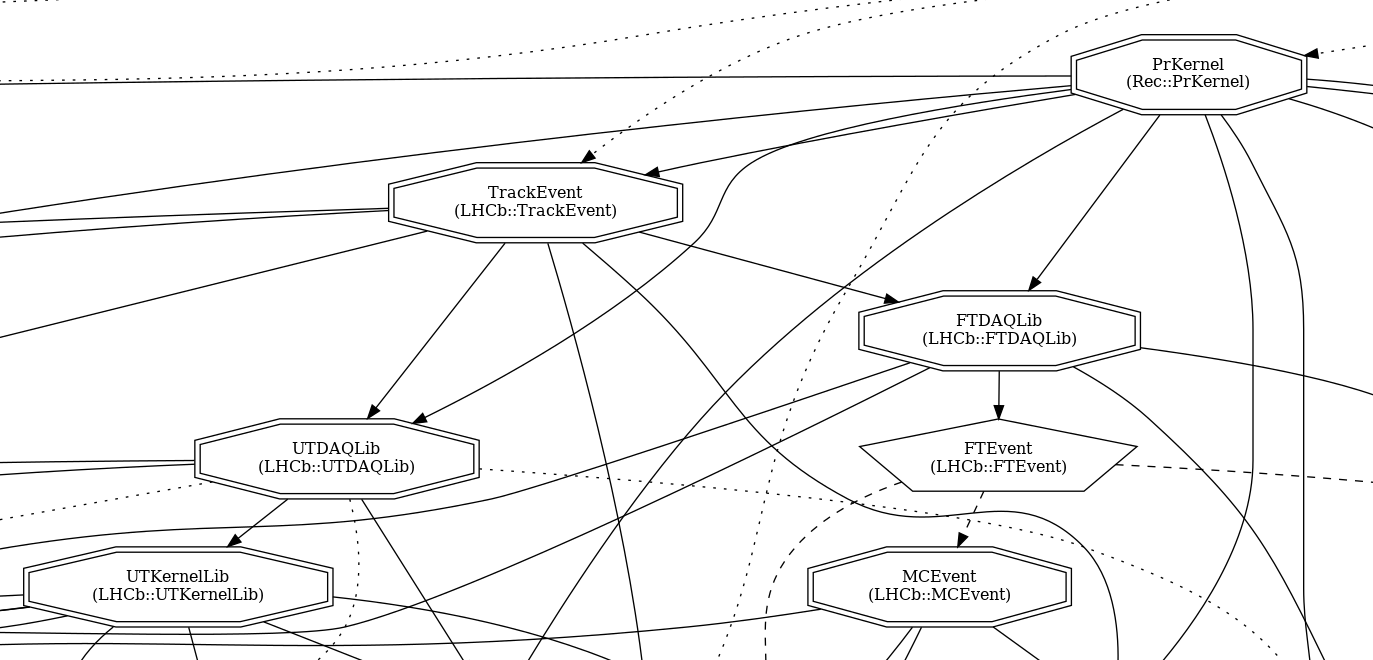
\includegraphics[width=\textwidth]{graphviz_cropped.png}
    \caption{Graphe des dépendances tracé avec graphviz}
    \label{Graphviz}
\end{figure}

\subsection{Passage des bibliothèques partagées en bibliothèques statiques}
Intéressons-nous au remplacement des bibliothèques partagées par des bibliothèques statiques.

C'est le code CMake qui compile le code, crée les bibliothèques et les link.
Ainsi, dans le programme Gaudi, il y a déjà des fonctions CMake qui permettent de facilement créer des bibliothèques partagées, \verb'gaudi_add_library', et des modules, \verb'gaudi_add_module'.
Il est donc simple de copier la fonction \verb'gaudi_add_library', qui crée une bibliothèque partagée, en une fonction \verb'gaudi_add_static_library'.
Cette fonction utilise la fonction CMake \verb'add_library' dans laquelle il suffit de changer le paramètre \verb'STATIC' en \verb'SHARED'.

Avec cette nouvelle fonction, il est désormais facile de remplacer les bibliothèques partagée de la pile LHCb en bibliothèques statiques.

Cependant, à cette étape là, on peut se retrouver dans un cas où une bibliothèque statique est linkée (et donc intégrée) à une bibliothèque dynamique ou à un module.
Or le principe d'une bibliothèque dynamique est que comme elle est chargée dynamiquement, elle peut se retrouver à plusieurs endroits dans la mémoire, elle doit donc être compilée en \emph{position-independant code} pour pouvoir fonctionner.
Ce n'est pas le cas d'une bibliothèque statique pour laquelle on sait à la compilation où son code machine sera en mémoire.
On doit rajouter l'option de compilation \verb'-fpic' pour compiler les bibliothèques statiques en position-independant code (on pourra l'enlever lorsque tout sera statique).

\subsection{Passage des modules en bibliothèques statiques}
Cherchons maintenant à rendre les modules statiques.

Gaudi propose également une fonction CMake \verb'gaudi_add_module'.
On peut donc simplement remplacer les appels à cette fonction par l'appel à la fonction précédemment créée \verb'gaudi_add_static_library'.
Il faut également linker ces nouvelles bibliothèques statiques avec l'exécutable.
Pour cela il suffit d'utiliser la fonction CMake \verb'target_link_libraries' sur l'exécutable.

Ceci compile, en revanche il y a un problème à l'exécution.
En effet par défaut le linker supprime le code qui n'est pas utilisé.
Or jusqu'à présent, chaque module comprenait une partie qui était exécutée à son chargement et qui enregistrait le module dans une table.
En statique, cette fonction n'est donc pas utilisée et est donc supprimée.
De ce fait l'exécutable ne sait pas que le module est déjà chargé.

Résoudre ce problème correctement consisterait à revoir en profondeur ce système, ce qui semble trop complexe à ce stade.
La solution retenue a été d'utiliser l'option de linkage \verb'-Wl,--whole-archive' qui force le linker à garder l'ensemble du code.
Cependant avec cela des symboles sont inclus plusieurs fois ce qui mène à une erreur que l'on peut désactiver avec \verb'-Wl,--allow-multiple-definition'.
Il n'est normalement pas recommandé d'utiliser ses options car elles ne correspondent pas au comportement usuel du linker et peuvent donc être à l'origine de bugs ou de mauvaises optimisations.

Un autre problème est que l'on charge toujours dynamiquement quelques modules, notamment des foncteurs.
Or ceci ont besoin des symboles définis dans les bibliothèques désormais statiques et qui ne sont donc plus visibles.
Il faut donc activer l'option \verb'-Wl,--export-dynamic' pour résoudre cet autre problème.


\section{Guided optimization}

\subsection{Profile-guided optimization}
\subsubsection{Mise en place}
Le profile-guided optimization est inclus dans gcc et dans clang.
Pour cela il faut utiliser l'option de compilation \verb'-fprofile-generate' qui va permettre de compiler une version du programme avec instrumentation.

Ainsi, lorsqu'on va faire tourner le programme, des fichiers de profiles vont être générés, ils correspondent à des compteurs qui permettent de connaître l'utilisation de chaque fonction et branchement.

Ensuite pour compiler le programme final, il faut utiliser l'option \verb'-fprofile-use' pour utiliser les profiles.
On peut aussi rajouter l'option \verb'-fprofile-correction' pour corriger certains problèmes qui peuvent apparaître avec le \emph{multi-threading}.

Ces options sont mis de manière globale sur l'ensemble du projet CMake.

\subsubsection{Difficultés}
Le profile-guided optimization n'a d'abord pas donné de résultats, la vitesse d'exécution ne changeant pas.
C'est après un certain temps que l'on a compris que le PGO n'est efficace que si le \emph{link-time optimization} est également activé.

\subsection{AutoFDO}
Même si le principe général est similaire, la mise en place de AutoFDO diffère du PGO.

Tout d'abord la première compilation se fait normalement.

C'est ensuite lorsqu'on exécute le programme qu'on doit le faire en utilisant un outil de profiling.
Le plus simple à utiliser sous Linux est \verb'perf', cependant ceci nécessite d'avoir certains droits sur le système.
\begin{lstlisting}[language=bash]
perf -b -e br_inst_retired.near_taken:pp -- run_command
\end{lstlisting}
Il faut ensuite convertir les fichiers :
\begin{lstlisting}[language=bash]
create_gcov --binary=path/to/binary -- profile=perf.data --gcov=perf.gcov -gcov_version=1
\end{lstlisting}

Enfin on recompile l'exécutable avec l'option \verb'-fauto-profile=perf.gcov'.

Aucun résultat n'a pu être obtenu avec AutoFDO, on a donc abandonné l'utilisation de cet outil lorsque le PGO a donné des résultats.
On a pas trouvé la raison de cela, mais l'hypothèse la plus probable est que \verb'create_gcov' n'arrive pas à convertir correctement les données issues de \verb'perf'.

\subsection{Link-time optimization}
La mise en place du link-time optimization se fait à deux moments différents.
Tout d'abord au moment de la compilation des fichiers source en fichiers objets.
Puis au moment du link.
Avec gcc, cela se fait dans les deux cas via l'option \verb'-flto'.

Cependant dans CMake, il y a une meilleure manière de faire :
\begin{lstlisting}[language=bash]
include(CheckIPOSupported)
check_ipo_supported()
set(CMAKE_INTERPROCEDURAL_OPTIMIZATION TRUE)
\end{lstlisting}
Ici, on commence par vérifier que l'\emph{interprocedural optimization} (synonyme de link-time optimization) est supportée, puis on l'active de manière globale.
Cette solution a l'avantage de laisser CMake mettre en place le LTO pour la compilation et le link.

On peut remarquer que ceci augmente encore plus le temps de construction des programmes (environ $50\%$).

\subsection{VTune}
L'outil VTune créé par \emph{Intel} permet de comprendre l'utilisation du processeur par un programme.
On peut notamment voir le taux de mauvaises prédictions de branchement ou le temps que le processeur passe à attendre la mémoire.

\begin{figure}[H]
    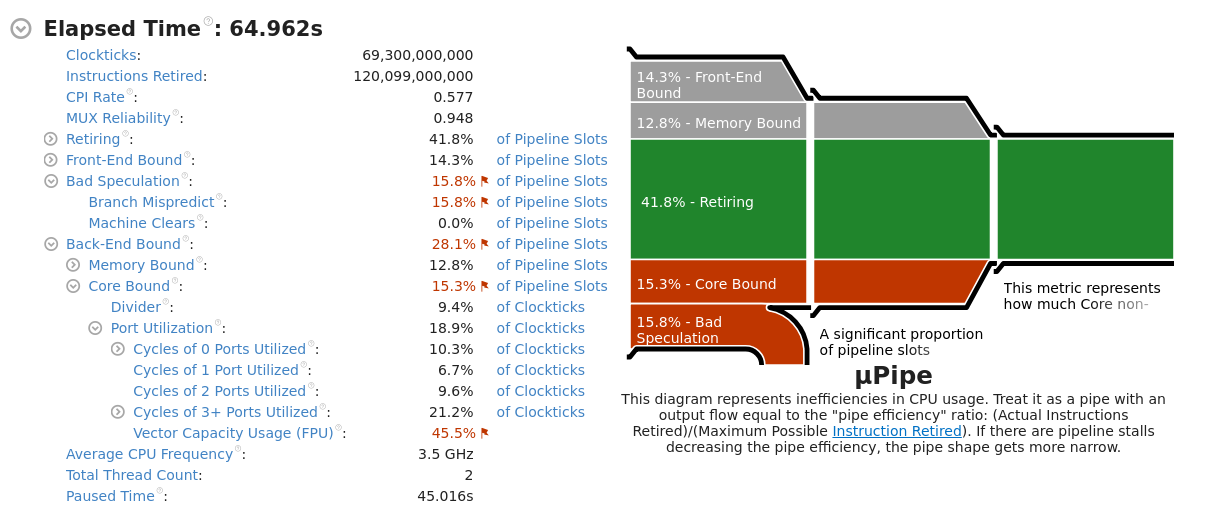
\includegraphics[width=\textwidth, center]{vtune_hlt1.png}
    \caption{Résumé de VTune pour le test \emph{Hlt1}}
    \label{vtune_hlt1}
\end{figure}

\begin{figure}[H]
    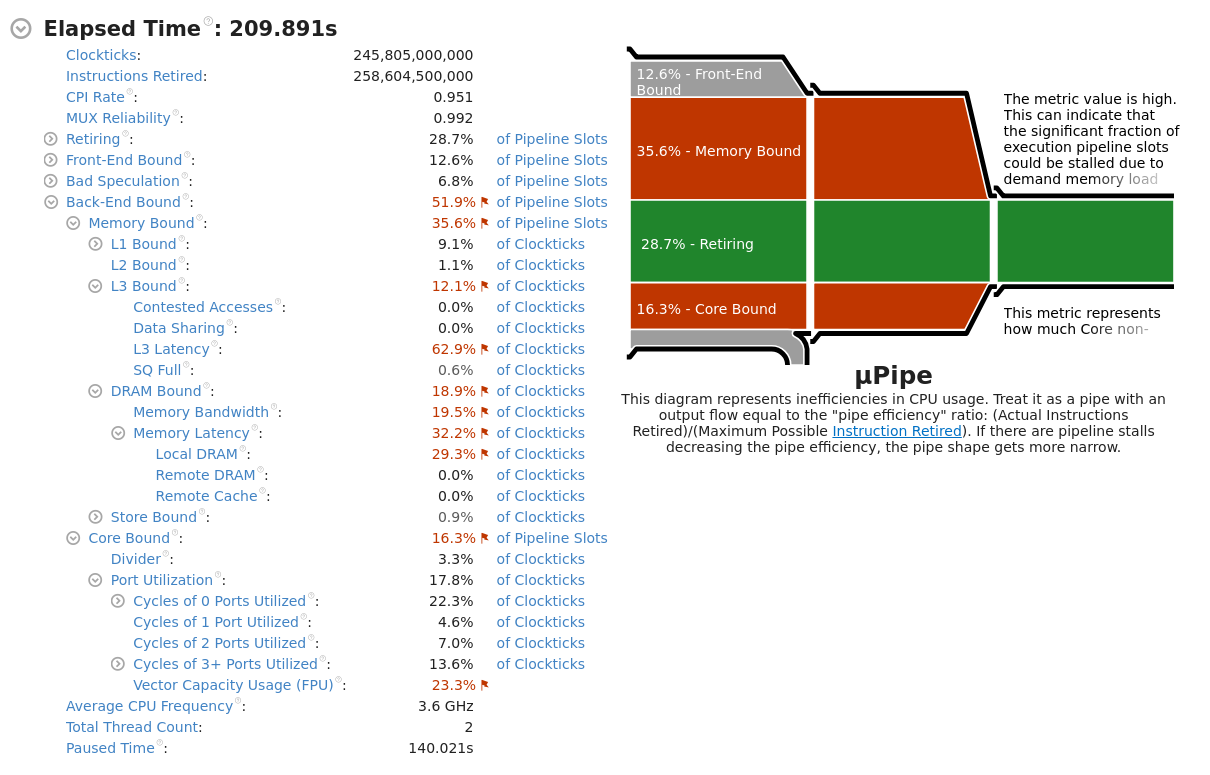
\includegraphics[width=\textwidth, center]{vtune_hlt2.png}
    \caption{Résumé de VTune pour le test \emph{Hlt2}}
    \label{vtune_hlt2}
\end{figure}

On peut remarquer que le test \emph{Hlt1} optimise de base beaucoup mieux l'utilisation du processeur que le test \emph{Hlt2}.

\section{Include-what-you-use}
\emph{iwyu} a été conçu pour fonctionner avec \emph{clang} et \emph{llvm}.
Encore une fois, il est aisé d'utiliser cet outil à travers CMake.
En effet il suffit de donner à la variable \verb'CMAKE_CXX_INCLUDE_WHAT_YOU_USE' la commande faisant tourner \verb'include-what-you-use'.
Il faut alors faire tourner CMake avec la version de clang correspondante comme compilateur.

Il y avait une version du programme compatible avec \verb'clang12' installé sur le système.
Cependant, il y a rapidement eu un bug, l'outil gérant mal certaines références cycliques.
Après recherche, ce bug n'a été corrigé qu'avec la dernière version de iwyu, qu'il a donc fallut télécharger et recompiler avec \verb'clang16'.

L'outil a alors correctement pu tourner.
En revanche on a alors remarqué qu'il y avait toujours des bugs, notamment il supprimait parfois des inclusions en faite nécessaire ou en rajoutait qui ne servaient pas directement.
De plus, on a pu se rendre compte que certaines architecture utilisés, comme les fichiers contenant le code de \emph{templates}, étaient incompatibles avec le principe de l'outil.

Finalement, la mise en place de include-what-you-use a été abandonnée et n'a servi qu'à repérer et corriger quelques erreurs déjà présentes.

\section{Fast-math et stabilité numérique}
\subsection{Comparaison flottante}
\subsubsection{Test d'égalité}
Les nombres flottants étant des approximations, la notion d'égalité n'a pas vraiment de sens.
Cependant l'opérateur de test d'égalité est défini pour les flottants en C et en C++.
Celui-ci vaut vrai si les deux nombres sont strictement les mêmes.
On peut aussi préciser que \verb'-0.0 == +0.0' est vrai tandis que \verb'NaN' n'est pas égal à lui-même.

Pour repérer les tests d'égalité, on peut utiliser l'option de compilation \verb'-Wfloat-equal' qui imprime un \emph{Warning} pour chaque test d'égalité.
Remplacer ces tests par d'autres tenant compte d'une erreur est important car sinon un simple arrondi peut faire basculer leurs résultats.

\subsubsection{Validité d'une division}
La division par zéro étant impossible, il faut trouver un moyen de gérer ce cas en informatique.

Pour cela on trouve parfois ce genre de code.
\begin{lstlisting}[language=c++]
if (f(x) != 0.)
    return 5./f(x);
else
    ...
\end{lstlisting}
Cependant ici \verb'f(x)' est calculé deux fois et il se pourrait très bien que la première fois son résultat soit proche de zéro sans en être égal, tandis que la deuxième fois le résultat soit $0$.
Cela peut arriver si par exemple le compilateur décide d'utiliser du \emph{FMA} (jeu d'instructions pour le calcul flottant) pour l'un des deux calculs mais pas l'autre, l'arrondi pouvant être différent.
Ainsi le test passerait et on diviserai pas zéro.

Une autre solution serait de tenter de ne calculer qu'une seule fois \verb'f(x)'.
\begin{lstlisting}[language=c++]
float y = f(x);
if (y != 0.)
    return 5./y;
else
    ...
\end{lstlisting}
Mais en fait cela ne change rien car le compilateur peut décider de toujours faire le calcul deux fois (à moins d'utiliser \verb'volatile'), si par exemple il estime que c'est plus rapide que de passer par la mémoire.
De plus, même si $f(x)$ ne vaut pas $0$, s'il en est suffisamment proche, \verb'5./f(x)' peut valoir \verb'+Inf'.

Une solution plus robuste au problème est de faire la division puis de vérifier après coup qu'elle s'est bien passée.
Pour cela on peut utiliser \verb'isfinite'.
\begin{lstlisting}[language=c++]
float result = 5./f(x);
if (std::isfinite(result))
    return result;
else
    ...
\end{lstlisting}
Cela à l'avantage de fonctionner peu importe l'opération ou fonction mathématique, et dans le cas d'un enchaînement de calculs on peut faire un seul test sur le résultat final.

Il est également possible d'utiliser le mécanisme de trapping qui permet d'exécuter une interruption par exemple en cas de division par zéro ou de dépassement.
Mais cette méthode se met en place à l'échelle du programme et ne devrait plus être utilisée de nos jours.

\subsection{Fast-math}
On peut activer fast-math en compilant avec l'option \verb'-ffast-math', mais cela ne fait qu'activer d'autres options.

\subsubsection{no-math-errno}
Cette option permet de ne pas définir la valeur de la variable \verb'errno' après l'appel de fonctions pouvant être exécutées en une instruction (comme \verb'sqrt').
Ce mécanisme de gestion des exceptions ne devrait plus être réellement utilisé en C++ moderne, le désactiver n'est donc pas réellement problématique.

\subsubsection{no-signaling-nans}
Il existe un mécanisme permettant de remonter un signal lorsqu'un calcul est effectué avec une valeur \verb'NaN' comme opérande.
Cette option permet donc de ne pas générer de signal dans un certain nombre de cas.
Celle-ci est activée par défaut.

\subsubsection{no-trapping-math}
Un autre mécanisme génère des interruptions lorsqu'il y a par exemple une division par 0 ou un dépassement (overflow).
Cette option compile en supposant que ces interruptions ne seront pas visibles.

\subsubsection{finite-math-only}
Active des optimisations qui supposent que tous les nombres sont finis (pas de $\pm$Inf ou de NaN).

Ceci peut avoir pour conséquence de remplacer les appels à \verb'isfinite' par \verb'true'.
La plupart des problèmes que l'on peut obtenir à cause de fast-math viennent de cette option pour cette raison.

\subsubsection{no-signed-zeros}
Le compilateur arrête de faire la différence entre $+0.0$ et $-0.0$.
Il peut ainsi simplifier des expressions comme \verb'0.0+x' en \verb'x'.

C'est probablement l'option la plus sûre à activer car peu d'algorithmes nécessitent que $0$ soit signé.

\subsubsection{associative-math}
Les flottants sont désormais considérés comme associatifs.
Cela permet de nombreuses optimisations :
\begin{enumerate}
    \item Simplification d'expressions comme \verb'2.0*x*3.0' en \verb'6.0*x' ;
    \item Meilleure vectorisation, c'est-à-dire utiliser des instructions du processeur permettant de faire un calcul sur plusieurs données à la fois.
          Par exemple \verb'((a*b)*c)*d' peut être changé en \verb'(a*b)*(c*d)' ce qui permet de calculer \verb'a*b' et \verb'c*d' en même temps.
    \item En réordonnant certains calculs, il est possible d'utiliser des jeux d'instruction du processeur comme le \emph{FMA}.
          Celui-ci permet par exemple de faire une multiplication suivie d'une addition en une seule instruction.
\end{enumerate}

Du fait de tous ces changements, les résultats des calculs peuvent changer.
Dans un certain nombre de cas ils peuvent être plus justes du fait du FMA qui est plus précis et des simplifications qui en réduisant le nombre de calculs limitent le nombre d'arrondis effectués.
Cependant il existe quelques algorithmes numériques qui reposent sur les règles d'arrondis et qui risquent donc de ne plus fonctionner correctement avec associative-math.

\subsubsection{reciprocal-math}
Pour la plupart des processeurs, il est plus rapide de calculer une multiplication qu'une division.
Ainsi, si on veut diviser plusieurs nombres par un même nombre $y$ (ce qui arrive typiquement lorsqu'on normalise un vecteur), il peut être plus intéressant de calculer une fois l'inverse de $y$ puis de le multiplier à chaque nombre que l'on veut diviser.

C'est ce que permet reciprocal-math qui va remplacer \verb'x/y' par \verb'x*(1/y)' lorsque cela permet un gain de temps.
Ceci peut engendrer une perte de précision.

\subsubsection{unsafe-math-optimizations}
Cette options active no-signed-zeros, no-trapping-math, associative-math, reciprocal-math ainsi que d'autre optimisations comme la non prise en charge des nombres dénormalisés (nombres très proches de $0$).

L'activer change des options du \emph{FPU} (unité de calcul des flottants) du processeur, ce qui peut impacter les autre bibliothèques chargées dynamiquement.
Il y a donc un effet de bord sur les autre bibliothèques qui peut être très difficile à débuguer.

\subsection{Mesure de l'instabilité}
En activant certaines de ces options, notamment no-signed-zeros, associative-math et reciprocal-math, on change légèrement la manière de faire certains calculs.
Ainsi, si ces petites différences ont un impact important sur les résultats finaux, cela veut dire que nos algorithmes sont probablement instables numériquement et qu'il faudrait les corriger.

L'infrastructure LHCb possède déjà un grand nombre de compteurs qui représentent des résultats d'algorithmes.
Ils sont notamment utilisés pour effectuer des tests et permettent donc de repérer si les modifications du code changent leurs valeurs.
Ainsi, il a été possible via un code Python de récupérer ces compteurs et les enregistrer au format \verb'csv'.
On peut ensuite ouvrir ce fichier avec un logiciel de tableur afin de mesurer l'erreur relative entre la référence et la version fast-math et d'en faire des statistiques.

Ainsi on peut voir quels sont les algorithmes les plus sensibles aux options de fast-math et donc probablement numériquement instables.


\chapter{Résultats}

\section{Amélioration de la rapidité d'exécution}
Pour mesurer les améliorations, des \emph{throughput test} ont été faits.
\emph{Hlt1} a été testé sur la version statique et PGO, mais aucune amélioration n'a été observée.
Voici les résultats pour le test \emph{Hlt2} :

\begin{center}
    \begin{tabular}{ c c c }
        Optimisation                           & Amélioration & Intervalle de confiance ($2\sigma$) \\
        LTO                                    & $0.17\%$     & $\pm 1.12\%$                        \\
        LTO \& PGO                             & $6.74\%$     & $\pm 1.44\%$                        \\
        Static LTO                             & $0.87\%$     & $\pm 0.60\%$                        \\
        Static LTO \& PGO                      & $6.88\%$     & $\pm 0.83\%$                        \\
        Fast-math\footnotemark[1]              & $5.06\%$     & $\pm 0.98\%$                        \\
        Associative-math seulement             & $4.73\%$     & $\pm 1.51\%$                        \\
        Fast-math\footnotemark[1] + LTO \& PGO & $11.02\%$    & $\pm 0.98\%$
    \end{tabular}

    \footnotetext[1]{sans finite-math-only et unsafe-math-optimizations}
\end{center}

\section{Bibliothèques statiques}
L'exécutable final passe de $\sim 20 Ko$ à $2,5 Go$.

On remarque qu'utiliser des bibliothèques statiques à la place des dynamiques ne change pas significativement la rapidité.
En revanche on a bien vu que cela pouvait entraîner des bugs supplémentaires, notamment avec les foncteurs.

\section{Guided optimization}
\subsection{Gain}
Il y a un net gain de performance à utiliser le profile-guided optimization et le link-time optimization (environ $7\%$ d'amélioration).
Ceci peut représenter plusieurs milliers de machines à l'échelle des centres de calculs du LHCb.

\subsection{Code final}
Le code finalement ajouté au CMake global du projet est :
\begin{lstlisting}[language=make,numbers=left]
if("${PGO}" MATCHES "GENERATE")
	message("PGO generate")
	if(DEFINED PGO_PATH)
		set(CMAKE_CXX_FLAGS "${CMAKE_CXX_FLAGS} -fprofile-generate=${PGO_PATH}")
	else()
		set(CMAKE_CXX_FLAGS "${CMAKE_CXX_FLAGS} -fprofile-generate")
	endif()
endif()
if("${PGO}" MATCHES "USE")
	message("PGO use")
	if(DEFINED PGO_PATH)
		set(CMAKE_CXX_FLAGS "${CMAKE_CXX_FLAGS} -fprofile-use=${PGO_PATH} -fprofile-correction")
	else()
		set(CMAKE_CXX_FLAGS "${CMAKE_CXX_FLAGS} -fprofile-use -fprofile-correction")
	endif()
	include(CheckIPOSupported)
	check_ipo_supported()
	set(CMAKE_INTERPROCEDURAL_OPTIMIZATION TRUE)
endif()
\end{lstlisting}

\subsection{Mise en production}
En l'état il n'est pas évident de mettre en production une version PGO.
En effet les programmes sont pour l'instant compilés et installés un à un.
Or le PGO nécessite de tout compiler une fois pour pouvoir faire tourner le programme.
Il faudrait donc changer la manière d'installer les programmes pour utiliser plus simplement cette version.

\section{Fast-math}
Après quelques tests, il a été décidé de ne pas utiliser finite-math-only car il y a un certain nombre d'endroits dans le code qui utilisent des flottants non-finis.
De même pour unsafe-math-optimization qui a des effets de bords subtiles sur les bibliothèques chargées dynamiquement.

\subsection{Gain}
On observe que fast-math permet un important gain de performance (environ $5\%$ d'amélioration).
De plus, il se cumule presque avec celui du PGO qui lorsqu'on les utilisent ensembles, permettent d'obtenir une amélioration de plus de $10\%$.

On remarque également que ce gain vient surtout d'associative-math, les autres options n'ont donc pas beaucoup d'effet.
Plus précisément, on peut utiliser VTune pour voir le temps que passe le processeur à faire des calculs sur flottants.

\begin{figure}[!htb]
    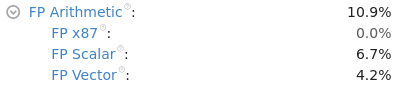
\includegraphics[width=0.5\textwidth, center]{reference_vtune.png}
    \caption{Référence}
    \label{reference_vtune}
\end{figure}

\begin{figure}[!htb]
    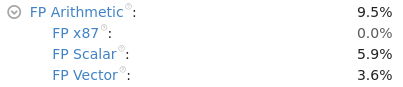
\includegraphics[width=0.5\textwidth, center]{associative-math_vtune.png}
    \caption{Associative-math}
    \label{associative-math_vtune}
\end{figure}

On observe sur les figures \ref{reference_vtune} et \ref{associative-math_vtune} qu'avec associative-math, le processeur réduit d'environ $10\%$ le temps passé dans l'unité de calculs flottants.

\subsection{Mesure de l'instabilité}
On peut voir sur la figure \ref{fast-math_difference} qu'un certain nombre de compteurs ont une différence significative avec la référence.
En effet on considère que lorsque l'erreur relative dépasse $10^{-4}$ voire $10^{-3}$, l'erreur est trop importante pour la physique.

On obtient le même graphique en comparant la version associative-math avec la référence.
Ainsi c'est le simple fait de changer l'ordre des opérations qui a un impact sur les résultats numériques.

\begin{figure}[!htb]
    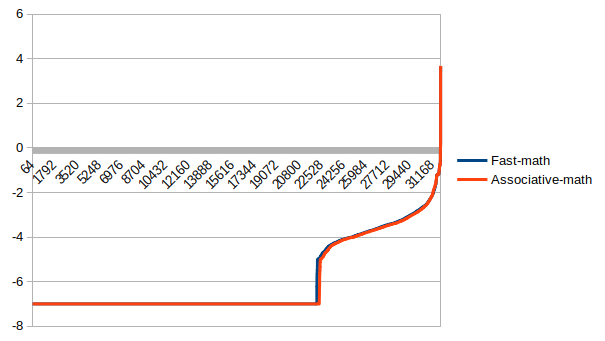
\includegraphics[width=\textwidth, center]{fast-math_difference.png}
    \caption{Logarithme de l'erreur relative des compteurs entre la référence et la version fast-math}
    \label{fast-math_difference}
\end{figure}

\section{Réflexions sur la responsabilité sociétale et environnementale}
Le CERN est une organisation internationale faisant de la recherche, il n'est pas à but lucratif.
Si les états membres investissent des milliards c'est parce qu'il est probable que dans plusieurs décennies, les découvertes qui y sont faites auront un grand impacte sur nos sociétés,
comme a pu l'être la physique quantique qui a par exemple permis l'informatique ou toutes les technologies utilisant des lasers.
Il y a de fortes chances que ces découvertes concernent l'énergie.

Cependant, le CERN utilise un grand nombre d'installations qui peuvent avoir un impact sur l'environnement.
Le plus gros problème est la consommation électrique du LHC qui peut atteindre $200MW$, ce qui représente un tier de la consommation de Genève.
Cette électricité provient tout de même principalement de France et est donc en large partie décarbonée.
Le CERN tente également de limiter sa consommation via différents moyens comme avec une utilisation plus importante des supraconducteurs au LHC ou la récupération de chaleur.
Les efforts en matière d'économies d'énergie ont permis au CERN d'être certifié ISO 50001.

Certaines des technologies développées au CERN peuvent être utilisées dans des domaines qui n'ont à priori rien à voir ;
une collaboration est par exemple en train de se mettre en place afin d'utiliser le programme ROOT (qui permet de calculer des trajectoires de particules) pour détecter les fraudes sur les marchés financiers.
Concernant les droits humains, avec l'invasion de l'Ukraine en 2022, le CERN a aussi décidé de mettre fin à la participation de la Russie et de la Biélorussie.


\chapter*{Conclusion}
\pagenumbering{gobble}
L'objectif de ce stage était de proposer et d'implémenter des solutions pour accélérer les programmes d'analyses de LHCb via des optimisations à la compilation.
Plusieurs résultats ont donc été obtenus.

Utiliser des bibliothèques statiques au lieu de bibliothèques dynamiques ne semble pas apporter d'avantage mais mène en revanche à de nombreux bugs.
Il ne semble donc pas intéressant de le mettre en place pour la suite.

Le profile-guided optimization apporte en revanche une accélération significative, on recommande donc de le mettre en place pour l'environnement de production.

On recommande également de créer une nouvelle platforme cible de compilation avec fast-math activé,
\begin{enumerate}
    \item dans un premier temps afin de pouvoir suivre l'instabilité numérique,
    \item dans un second temps pour utiliser fast-math en production, en complément du PGO.
\end{enumerate}

Ces optimisations permettraient d'atteindre plus de $10\%$ d'accélération pour les machines de productions.
Cela représente une économie en puissance de calcul d'environ $10\%$ des serveurs de production, soit plusieurs milliers de machines.
Celles-ci pourront donc être utilisées pour traiter plus de données.


\printbibliography

\end{document}
